\section{Appendix}

% \label{alg:fre-common}


\subsection{detailed experimental settings}

\subsubsection{System Auditing Collection}
Although \tool can handle input from Linux and Windows systems, our evaluation focuses primarily on Windows events. Because most of our benign deployment environment consists of Windows-based hosts, and sophisticated malware is mostly designed for Windows platforms, this is largely due to the fact that we have a benign deployment environment. We use \textit{Sysmon}, Windows' sophisticated log collection tool, to collect provenance data from these systems. System logs are captured thoroughly and exhaustively by leveraging \textit{Sysmon}'s default settings.

\subsubsection{Attack Datasets}

To address the challenges, we approache the problem from three distinct angles: expanding coverage of malicious functionalities and the ATT\&CK framework, employing advanced stealthy techniques, and simulating genuine APT attacks.

We executed our APT attack simulations in three steps:

\begin{itemize}
    \item  \textbf{Enhancing Malicious Functionalities:} In order to simulate a wider range of malicious activities, we handcrafted 14 malicious functions in C++, including BypassUAC, Encryption, File Monitor, Compression, Keyboard Monitor, and Privilege Escalation, etc. In addition, we implemented 9 different TTP attacks using well-known hacker utilities  \textit{Caldera}. Using C++ and \textit{Caldera} methodologies, we achieved 23 distinct malicious functions. APT attacks take place at various stages, including Initial Access, Privilege Escalation, Information Gathering, Defense Evasion, and ensuring Persistence.
    \item \textbf{Employing Stealth Techniques:} We incorporated four stealth methods: Process Masquerade, Process Hollow, Process Injection, and DLL Side-Loading. By combining these stealthy techniques with the 23 malicious functionalities, a variety of attack variants can be created. Process Masquerade and Process Hollow hide malicious process names, while Process Injection and DLL Side-Loading hide malicious DLLs.
    \item \textbf{Simulating Real-world APTs:} In order to enhance the authenticity of our simulations, we developed ten APT attack scenarios based on an analysis of real-world Advanced Persistent Threat activities. During a controlled testbed environment, audit logs were produced. We crafted ten simulated APT attack narratives using the four stealth techniques from the second step and the 23 malicious functionalities from the first step.
\end{itemize}

\noindent
{\bf Real-world datasets.} Using real-world datasets, we aimed to validate the frequency of masquerade techniques such as name masquerading in authentic APT attacks and associated malicious software; to this end, we collected publicly available APT attack simulation datasets alongside malware samples like GALLIUM\cite{cybereason2023}, DCSrv\cite{checkpoint2021}, and Egrego\cite{intrinsec}, etc. which are known to employ techniques like name masquerading and process injection;  APT29 poses as \textit{python.exe}, \textit{rar.exe}, and \textit{accesschk.exe}; furthermore, they utilize DLL Side-Loading, specifically by loading a malicious \textit{mso.dll} file, with comprehensive details showcased in the subsequent Table~\ref{tab:real_world}. We will delve into the specifics of how we utilized real-world datasets to validate the efficacy of our approach in Section~\ref{sec-real-world}.

\noindent
{\bf Label.}
By using our knowledge of attack workflow, we manually label the ground truth of interactions through their relation to attacks, as we are aware of how attacks are executed.


\subsubsection{Normal Datasets}
To validate the false positive rate of our methodology, A publicly available benign dataset, \cite{evtx-baseline2022}, is used in this analysis. This dataset encompasses logs generated from routine user activities across various Windows operating systems, including Windows 7, Windows 10 and Windows 11. The logs from this dataset cover the 13/47/52 processes for different system that we use to construct process profiles.

\begin{figure}[h]
    \centering
      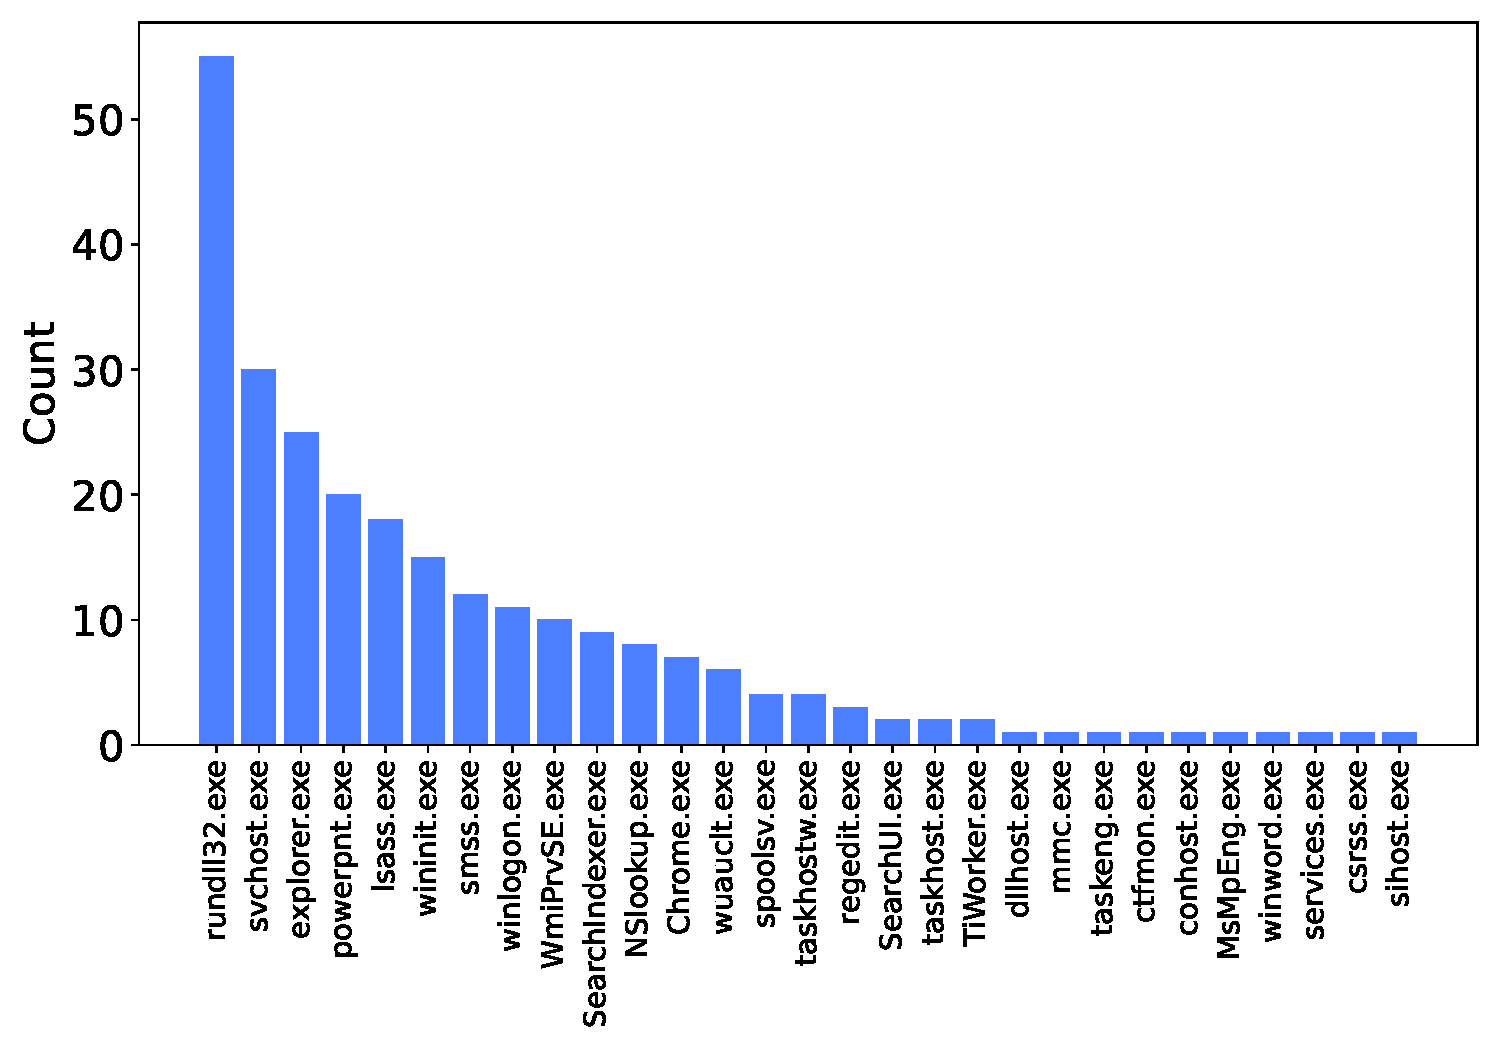
\includegraphics[width=0.45\textwidth]{figs/process.pdf}
    \caption{Comparison of attack frequencies for different processes based on the official MITRE website.}
    \label{fig-process}
\end{figure}

\subsubsection{Process Classification}
In order to construct a comprehensive analysis framework, we strategically selected 100 pivotal processes for examination. The selection criteria encompassed multiple dimensions, including: 1) Core system processes that are integral to system functionality; 2) Processes highly associated with security mechanisms; and 3) Processes commonly utilized by system administrators. Additionally, we integrated an assessment of processes that are frequently targeted in cyber-attacks, based on statistical analysis derived from MITRE's official website as shown in Figure~\ref{fig-process}.

We highlight the two most common processes: \textit{svchost.exe} and \textit{rundll32.exe}:
\begin{itemize}
    \item \textbf{\textit{Svchost.exe} processes}. \textit{svchost.exe} is a Windows system utility that runs multiple services from dynamic link libraries (.dll files). Given its trusted status and constant presence, adversaries often mimic \textit{svchost.exe} for attacks. The behavior tree for \textit{svchost.exe}, constructed based on our approach, is shown in the Figure~\ref{fig:behavior-tree}.
    \item \textbf{\textit{Rundll32.exe} processes}. \textit{rundll32.exe} loads specific functions from .dll files. Unlike \textit{svchost.exe}, it's more vulnerable, as attackers can create their own .dll for it. Due to its exploitability, \textit{rundll32.exe} is a prime target for malware impersonation. 
\end{itemize}



\subsection{Algorithm}

\begin{algorithm}
\caption{Common Items and SubSequences Mining}
\label{alg:fre-common}
\begin{algorithmic}[1]
\Require A set of log sequences \( \mathcal{D} \), threshold \( \theta=1 \)
\Ensure Common subsequences \( \mathcal{F} \)
\Statex
\Function{extractCommonItems}{$\mathcal{D}$}
    \State \( \text{items\_set} = \) set of items from the first sequence in \( \mathcal{D} \)
    \For{each sequence \(S\) in \(\mathcal{D}\) excluding the first one}
        \State \( \text{items\_set} = \text{items\_set} \cap \) set of items from \(S\)
    \EndFor
    \State \Return \( \text{items\_set} \) 
\EndFunction
\Statex
\Function{PrefixSpanMining}{$\mathcal{D}$, $\theta$}
    \State \( \text{Implement PrefixSpan or use an existing library} \)
    \State \( \mathcal{F} = \) sequences with frequency \( \geq \theta \)
    \State \Return \( \mathcal{F} \)
\EndFunction
\Statex
\Function{Mining}{$\mathcal{D}$, $\theta$}
    \State \( \mathcal{C} \) = \Call{extractCommonItems}{$\mathcal{D}$}
    \For{each sequence \(S\) in \(\mathcal{D}\)}
        \State Remove items from \(S\) not in \( \mathcal{C} \)
    \EndFor
    \State \( \mathcal{F} \) = \Call{PrefixSpanMining}{$\mathcal{D}$, $\theta$}
    \State \Return \( \mathcal{F} \)
\EndFunction
\end{algorithmic}
\end{algorithm}


\begin{table*}
    \centering
    \begin{tabular}{|l|l|l|p{6cm}|}
        \hline
        Masquerading Type & Malware/APT & Targeting process & Description \\
        \hline
        \multirow{2}{*}{Process Masquerading}
        & GALLIUM\cite{cybereason2023} & \textit{cmd.exe} & Attackers use a renamed \textit{cmd.exe} file to evade detection \\
        \cline{2-4}
        & DCSrv\cite{checkpoint2021} & \textit{svchost.exe} & Attackers masquerade as a legitimate \textit{svchost.exe} process to encrypt all computer volumes \\
        \cline{2-4}
        & APT29\cite{mitre_g0016} & \textit{svchost.exe/rar.exe} & Renaming these benign processes for use in various stages of the attack \\
        \hline
        \multirow{3}{*}{Dynamic-link Library Injection} & Aria-body\cite{checkpoint2020} & \textit{rundll32.exe/dllhost.exe} & Aria-body loader inject itself to another process \\
        \cline{2-4}
        & BlackEnergy\cite{fsecure2019} & \textit{svchost.exe} & The driver component injects the main DLL component into \textit{svchost.exe} \\
        \cline{2-4}
        & Sykipot\cite{att2023} & \textit{outlook/iexplore.exe} & The malware scans running processes for outlook or iexplore and injects a DLL \\
        \hline
        \multirow{2}{*}{Process Hollowing} & RCSession\cite{secureworks} & \textit{svchost.exe} & RCSession was launched from \textit{English.rtf} via a hollowed \textit{svchost.exe} \\
        \hline
        \multirow{2}{*}{Dll side-Loading} & APT3\cite{mitre_g0022} & \textit{Chrome.exe} & Attackers side load DLLs with a valid version of Chrome with their tools \\
        \cline{2-4}
        & APT29\cite{mitre_g0016} & \textit{Msoev.exe} & Attackers use a HTA file to drop three executables into the \%TEMP\% directory \\
        \hline
    \end{tabular}
    \caption{Real world APT Attack using steathy technical}
    \label{tab:real_world}
\end{table*}




\subsection{Prompt}


% \subsubsection{Initialization Behavior Tree Prompt}
% \label{prompt-init-tree}
% \begin{tabularx}{\textwidth}{|c|X|}
% \hline
% \multicolumn{2}{|c|}{\textbf{Input:} \colorbox{codegreen}{\{process\_name\}}} \\
% \multicolumn{2}{|c|}{\textbf{Output:} \colorbox{SoftRed}{\{behavior\_tree\}}for\colorbox{codegreen}{\{process\_name\}}} \\
% \hline
% \textbf{Role} & You are a security expert well-versed in the legitimate behavior of crucial Windows processes. Now, you are qualified to assist in constructing behavior trees for legal processes. \\
% \hline
% \textbf{Goal} & 
% Based on your domain expertise, create an initial \colorbox{SoftRed}{\{behavior\_tree\}} for \colorbox{codegreen}{\{process\_name\}}. 
% Please note that this is an introductory prompt; focus only on primary behaviors (e.g., 1.1, 2.1) without delving into sub-layers. And concentrate on major behaviors specific to the process.
% \\ 
% \hline
% \multirow{6}{*}{\textbf{Output Format}} & This is just a format, in reality there can be deeper and more numerous sub-behaviors: \\
% & \colorbox{lightgray}{1. basic profile} \\
% & 1.1. execution path \\
% & 1.2. parent and child processes \\
% & 1.3. permissions \\
% & \colorbox{lightgray}{2. Fundamental Behavior} \\
% & 2.1. xxxxx \\
% & 2.2. xxxxxx \\
% & 2.3. xxxxx \\
% & 2.3.1 xxxxx \\
% & 2.3.1.1 Some deeper behavior \\

% & \dots \\
% \hline
% \multirow{5}{*}{\textbf{Notes}} 
% & 1. Each token has a cost, so keep your output concise and avoid irrelevant information. \\
% & 2. Continuously review and analyze your actions to ensure you are performing to the best of your abilities. \\
% & 3. Constructively self-criticize your big-picture behavior constantly. \\
% & 4. Ideally, behaviors should be generated that can be confirmed through system commands. \\
% \hline
% \textbf{\colorbox{codeorange}{LLM Response}} \\
% & \colorbox{lightgray}{1. basic profile} \\
% & 1.1. execution path: \colorbox{codeorange}{C:/Windows/System32/svchost.exe} \\
% & 1.2. Parent and Child Processes: Parent process is usually \colorbox{codeorange}{services.exe}. Child processes can vary based on the specific service \\
% & 1.3. Permissions: svchost.exe typically runs with system-level permissions \\
% & \colorbox{lightgray}{2. Fundamental Behavior} \\
% & 2.1. Service Hosting: Hosts multiple Windows operating system services \\
% & 2.2. Dynamic Link Library Loading: Loads DLL files that contain the actual code for the service \\
% & 2.3. Network Communication: Depending on the service, it may communicate over the network \\
% & 2.4. System Resource Management: Manages system resources such as memory and CPU for the services it hosts. \\
% \\
% \hline
% \end{tabularx}

% \clearpage
% \subsubsection{Expansion Behavior Tree Prompt}
% \label{prompt-expan-tree}

% \begin{tabularx}{\textwidth}{|c|X|}
% \hline
% \multicolumn{2}{|c|}{\textbf{Input:} \colorbox{SoftRed}{\{behavior\_tree\}}for\colorbox{codegreen}{\{process\_name\}}} \\
% \multicolumn{2}{|c|}{\textbf{Output:} \colorbox{SoftRed}{\{behavior\_tree\}}for\colorbox{codegreen}{\{process\_name\}}} \\
% \hline
% \textbf{Role} & You are a security expert well-versed in the legitimate behavior of crucial Windows processes. Now, you are qualified to assist in constructing behavior trees for legal processes. \\
% \hline
% \textbf{Goal} & 
% Based on the current knowledge, please update the original \colorbox{SoftRed}{\{behavior\_tree\}}.
% Please review the tree and determine if further refinement or subdivision is required for the current behaviors listed under the last branch. If, based on your expertise, no further details are needed for a specific behavior, please end the branch..
% \\ 
% \hline

% \multirow{5}{*}{\textbf{Notes}} 
% & 1. Each token has a cost, so keep your output concise and avoid irrelevant information. \\
% & 2. Continuously review and analyze your actions to ensure you are performing to the best of your abilities. \\
% & 3. Constructively self-criticize your big-picture behavior constantly. \\
% & 4. The best would be to generate behaviors that can be verified within the system command. \\
% \hline

% \textbf{\colorbox{codeorange}{LLM Response}} \\
% & \colorbox{lightgray} {2.1. Service Hosting: "Hosts multiple Windows services in the form of dynamic-link libraries (DLLs)} \\
% & 2.1.1 DHCP Client Service": "Obtains an IP address and other related information from a DHCP server \\
% & 2.1.1.1. IP Address Request": "Sends a request to the DHCP server to obtain an IP address \\
% & 2.1.1.2. IP Address Renewal": "renew the lease on the current IP address \\
% & .......\\
% & 2.1.2. DNS Client Service": "Resolves and caches Domain Name System (DNS) names \\
% & .... \\
% & 2.1.7. Remote Procedure Call (RPC) Service": "Provides the endpoint mapper and other miscellaneous RPC services\\
% \\
% \hline
% \end{tabularx}

% \clearpage

% \subsubsection{Commands Generation Prompt}
% \label{prompt-commands}

% \begin{tabularx}{\textwidth}{|c|X|}
% \hline
% \multicolumn{2}{|c|}{\textbf{Input:} \colorbox{SoftRed}{\{behavior\_tree\}}for\colorbox{codegreen}{\{process\_name\}}} \\
% \multicolumn{2}{|c|}{\textbf{Output:} \colorbox{LightPeach}{\{commands\}}for\colorbox{codegreen}{\{process\_name\}}} \\
% \hline
% \textbf{Role} & You are an expert in cybersecurity, proficient in understanding the legitimate behaviors of crucial Windows processes. You specialize in generating corresponding commands based on the behavior tree of the current process. \\
% \hline
% \textbf{Goal} &  \\
% & You are a cybersecurity specialist well-versed in the legitimate behaviors of essential Windows processes. \\
% & You will receive a current behavior tree that consists of various behaviors and sub-behaviors \\
% & Each sub-behavior is followed by parentheses indicating whether it has been translated into a corresponding command. \\
% & There are two methods for validation: \\
% & 1 If a system command can be directly generated from the behavior, create the specific command and append it to the behavior tree like so: (Command: xxx). \\
% & 2 If a system command cannot be generated, provide a corresponding recommendation such as rebooting the system, and append it to the behavior tree like so: (Suggestion: Suggestion) \\

% \\ 
% \hline
% \multirow{5}{*}{\textbf{Notes}} 
% & 1. Each token has a cost, so keep your output concise and avoid irrelevant information. \\
% & 2. Continuously review and analyze your actions to ensure you are performing to the best of your abilities. \\
% & 3. Constructively self-criticize your big-picture behavior constantly. \\
% & 4. Ideally, behaviors should be generated that can be confirmed through system commands. \\
% \hline
% \textbf{\colorbox{codeorange}{LLM Response}} \\
% & ...... \\
% & C:/Windows/system32/svchost.exe -k appmodel -s StateRepository \\
% & C:/Windows/system32/svchost.exe -k dcomlaunch -s LSM \\
% & C:/Windows/system32/svchost.exe -k localService -s w32Time \\
% & Get-DhcpServer4Scope -ScopeID \\
% & Get-DhcpServerv4Lease IPAddress\\
% & ...... \\
% \\
% \hline
% \end{tabularx}

% \clearpage

% \subsubsection{Constraints Generation and Explanation}
% \label{prompt-cons-explain}

% \begin{tabularx}{\textwidth}{|c|X|}
% \hline
% \multicolumn{2}{|c|}{\textbf{Input:}  \colorbox{codegreen}{\{process\_behavior\_description\}}} \\
% \multicolumn{2}{|c|}{\textbf{Output:} \colorbox{LightPeach}{\{explanation\}}} \\
% \hline
% \textbf{Role} & You are an expert in cybersecurity, proficient in understanding the legitimate behaviors of crucial Windows processes. You specialize in generating corresponding commands based on the behavior tree of the current process. \\
% \hline
% \textbf{Goal} &  \\
% &  You are a seasoned security expert with a deep understanding of Windows system processes. \\
% & You will be presented with a \{process\_behavior\_description\}. \\
% & This description can convert a corresponding command that, when executed on a system, generates a log. \\
% & Analyze each log entry with a specific focus on: \\
% &   1 DLL meanings \\
% &    2 Registry key values meanings \\
% &   3 File names meanings  \\
% &    4 Process names meanings  \\
% & Relevance Levels: \\
% & 1 \{Essential\}   \\
% & 2 \{Strongly\_Related\}   \\
% & 3 \{Possibly\_Related\}  \\
% & 4 \{Unrelated\}   \\
% & For each log entry, categorize its relevance levels and provide an explanation for categories \{Essential\} 
% \\ 
% \hline
% \multirow{5}{*}{\textbf{Example}} 
% & Log Entry: RegQueryValue,hklm/system/currentcontrolset/control/scmconfig/*.\\
% & [RegQueryValue,hklm/system/currentcontrolset/control/scmconfig/*][Essential] [Explanation: The process frequently queries the Windows Registry to retrieve configuration or settings. The registry key path hklm/system/currentcontrolset/control/scmconfig* is associated with configurations related to the Service Control Manager (SCM).] \\
% & 3. Constructively self-criticize your big-picture behavior constantly. \\
% & 4. Ideally, behaviors should be generated that can be confirmed through system commands. \\
% \\
% \hline
% \end{tabularx}

% \subsubsection{Temporal Constraint Validation}
% \label{prompt-init-temporal}

% \begin{tabularx}{\textwidth}{|c|X|}
% \hline
% \multicolumn{2}{|c|}{\textbf{Input:} \colorbox{SoftRed}{\{log\_Sequence\}}for\colorbox{codegreen}{\{process\_name\}}} \\
% \multicolumn{2}{|c|}{\textbf{Output:} \colorbox{LightPeach}{\{These two logs must appear in this specific order.\}}for\colorbox{codegreen}{\{process\_name\}}} \\
% \hline
% \textbf{Role} & You are a security expert and will receive logs from a certain process. Using your expertise, determine if there is a sequential dependency between these logs. If such a dependency exists, please identify it and explain the rationale behind this relationship. \\
% \hline
% \textbf{Notes} &  \\
% & Analyze each log entry individually and pinpoint logs that must appear in a specific order. Refrain from providing superfluous explanations. \\
% \\ 
% \hline
% \textbf{\colorbox{codeorange}{LLM Response}} \\
% & [lsass.exe,Load,c:/windows/system32/lsasrv.dll, then Load, c:/windows/system32/samsrv.dll] \\
% & lsasrv.dll  serves as a core component of the LSA, and often needs to interact with SAM and samsrv.dll provides the essential interfaces and functions for interacting with the SAM database.
% \\
% \hline
% \end{tabularx}


% \clearpage
% \subsubsection{Cross-session Validation}
% \label{prompt-cross-validation}


% \begin{tabularx}{\textwidth}{|c|X|}
% \hline
% \multicolumn{2}{|c|}{\textbf{Input:} \colorbox{SoftRed}{\{process\_behavior\}}for\colorbox{codegreen}{\{process\_name\}}} \\
% \multicolumn{2}{|c|}{\textbf{Output:} \colorbox{SoftRed}{\{yes\}}or\colorbox{codegreen}{\{No\}}} \\
% \hline
% \textbf{Role} & You are Agent1, a cybersecurity specialist with expertise in legitimate behaviors of key Windows processes. There are a total of 3 agents. \\
% \hline
% \textbf{Goal} & 
% \\
% & We aim to verify the legitimacy of a program's behavior.\\
% &  To achieve this, different LLM sessions will debate the behaviors, ensuring their accuracy and consistency. \\
% & For the provided behaviors, explain their legitimacy. Why do you believe these behaviors are inherent to the process in question? \\
% & You will also receive feedback from other LLM sessions. The format is: \\
% & Agent 1: "This behavior is inherent to process XX because..." \\
% & Agent 2: "This behavior..." \\
% & ...... \\
% \\ 
% \hline

% \multirow{5}{*}{\textbf{Other Agent}} 
% & 1. You are Agent2, a cybersecurity specialist with expertise in legitimate behaviors of key Windows processes. There are a total of 3 agents.. \\
% & 2. You are Agent3, a cybersecurity specialist with expertise in legitimate behaviors of key Windows processes. There are a total of 3 agents. \\
% \hline

% \multirow{5}{*}{\textbf{Notes}} 
% & 1. Keep your answer as concise as possible, just yes or no, and follow it up with the reason why \\
% & 2. After engaging in several rounds of debate, if you are confident in your assessment, please respond with "yes". \\
% \hline

% \textbf{\colorbox{codeorange}{LLM Response}} \\
% & \colorbox{lightgray} {xxx} \\
% \\
% \hline
% \end{tabularx}




